\documentclass[conference]{IEEEtran}
\IEEEoverridecommandlockouts
% The preceding line is only needed to identify funding in the first footnote. If that is unneeded, please comment it out.
\usepackage{cite}
\usepackage{amsmath,amssymb,amsfonts}
\usepackage{algorithmic}
\usepackage{graphicx}
\usepackage{textcomp}
\usepackage{xcolor}
\usepackage[brazilian]{babel}
\usepackage[utf8]{inputenc}
\usepackage[T1]{fontenc}
\def\BibTeX{{\rm B\kern-.05em{\sc i\kern-.025em b}\kern-.08em
    T\kern-.1667em\lower.7ex\hbox{E}\kern-.125emX}}
\begin{document}

\title{Algoritmos Genéticos}

\author{Bruno Lopes}
\maketitle

\section{INTRODUÇÃO}
Os algoritmos genéticos \cite{b1} são uma família de modelos computacionais inspirados na teoria da evolução Darwiniana \cite{b2}, no qual existe inicialmente um conjunto de indivíduos (população inicial), que incorporam uma solução potencial para um problema específico numa estrutura semelhante a de um cromossomo e aplicam operadores de seleção e "cross-over" a essas estruturas de forma a preservar informações críticas relativas à solução do problema.
    
O algoritmo genético (AG) foi apresentado inicialmente por John Holland em seu trabalho intitulado de “Adaptation in Natural and Artificial Systems” em 1975, com o objetivo de  formalizar  matematicamente  e  explicar  os  processos  de  adaptação  de  processos  naturais e  desenvolver  sistemas  artificiais  que  mantenham  os  mecanismos  originais  encontrados  em sistemas naturais \cite{b3}. 

Uma das vantagens de um AG é a simplificação que eles permitem na formulação e solução de  problemas de otimização. AG's simples normalmente trabalham com descrições de entrada formadas por cadeias de bits de tamanho fixo. Outros tipos de AG's podem trabalhar com cadeias de bits de tamanho variável, como por exemplo AG's usados para Programação Genética. 

Uma implementação de um algoritmo genético começa com uma população aleatória de cromossomos. Essas estruturas são, então, avaliadas e associadas a uma probabilidade de reprodução de tal forma que as maiores probabilidades são associadas aos  cromossomos que representam uma melhor solução para o problema de otimização do que àqueles que representam uma solução pior. A aptidão da solução é tipicamente definida com relação à população corrente.

A função objetivo de um problema de otimização é construída a partir dos parâmetros envolvidos no problema. Ela fornece uma medida da proximidade da solução em relação a um conjunto de parâmetros. Os parâmetros podem ser conflitantes, ou seja, quando um aumenta o outro diminui. O objetivo é encontrar o ponto ótimo. A função objetivo permite o cálculo da aptidão bruta de cada indivíduo, que fornecerá o valor a ser  usado para o cálculo de sua probabilidade de ser selecionado para reprodução.

\section{Referencial Teórico}

Algoritmos Genéticos são algoritmos de otimização global, baseados nos mecanismos de seleção natural e da genética \cite{b2}. Eles empregam uma estratégia de busca paralela e estruturada, mas aleatória, que é voltada em direção ao reforço da busca de pontos de "alta aptidão", ou seja, pontos nos quais a função a ser minimizada (ou maximizada) tem valores relativamente baixos (ou altos).

Os princípios da natureza nos quais os GAs se inspiram são simples. De  acordo com  a teoria de C. Darwin, o princípio de seleção privilegia os indivíduos mais aptos com maior longevidade e, portanto, com maior probabilidade de reprodução. Indivíduos  com  mais descendentes têm mais chance de perpetuarem seus códigos genéticos nas próximas   gerações.

Os algoritmos genéticos foram introduzidos por J. Holland em 1975 \cite{b1} com o objetivo de formalizar matematicamente e explicar rigorosamente processos de adaptação em sistemas naturais e desenvolver sistemas artificiais artificiais (simulados em computador) que retenham os mecanismos originais encontrados em  sistemas  naturais. 

Em 1975, Holland publicou o livro Adaptation in Natural and Artificial Systems, hoje considerado a Bíblia de Algoritmos Genéticos. Desde então, estes algoritmos vêm sendo aplicados com sucesso nos mais diversos problemas de otimização e aprendizado de máquina. 

Os AG's possuem uma larga aplicação em muitas áreas científicas, entre as quais podem ser destacadas:
    
    \begin{itemize}
    \item Síntese de circuitos analógicos:  para uma certa entrada e uma saída desejada, por exemplo tensão, o AG gera a topologia , o tipo e o valor dos componentes do circuito.

    \item Síntese de protocolos:  determinação de quais funções do protocolo devem ser implementadas em hardware e quais devem ser implementadas em software para que um certo desempenho seja alcançado.

    \item Programação Genética: gera a listagem de um programa, numa determinada linguagem especificada, para que um determinado conjunto de dados de entrada forneça uma saída desejada.

    \item Gerenciamento de redes: supervisão do tráfego nos links e das filas nos "buffers" de roteadores para descobrir rotas ótimas e para reconfigurar as rotas existentes no caso de falha de algum link.

    \item Computação Evolutiva: gera programas que se adaptam a mudanças no sistema ao longo do tempo.

    \item Otimização evolutiva multi-critério: otimização de funções com múltiplos objetivos que sejam conflitantes.

    \item Problemas de otimização complexos: problemas com muitas variáveis e espaços de soluções de dimensões elevadas. Ex: problema do caixeiro viajante, gerenciamento de carteiras de fundos de investimento.

    \item Ciências biológicas:  modela processos biológicos para o entendimento do comportamento de estruturas genéticas.

    \item Autômatos auto-programáveis.
    \end{itemize}

A idéia básica de funcionamento dos algoritmos genéticos é a de tratar as possíveis soluções do problema como "indivíduos" de uma "população", que irá "evoluir" a cada iteração ou "geração". Para isso é necessário construir um modelo de evolução onde os indivíduos sejam soluções de um problema. 

 A estrutura geral do programa está apresentada na Figura1 e os detalhes da execução do algoritmo pode ser resumida nos seguintes passos:
    \begin{itemize}
    \item População inicial, normalmente formada por indivíduos criados aleatoriamente;
    Avaliar a população de indivíduos segundo algum critério de qualidade (função de aptidão ou "fitness");
    
    \item Em seguida, através do operador de "seleção", escolhem-se os indivíduos de mais aptos com maior longevidade para a criação de um novo conjunto de possíveis soluções, chamado de nova "geração";
    
    \item Esta nova geração é obtida aplicando-se sobre os indivíduos selecionados operações que misturem suas características (chamadas "genes"), através dos operadores de "cruzamento" ("crossover") e "mutação";
    
    \item Estes passos são repetidos até que uma solução aceitável seja encontrada, até que o número predeterminado de passos seja atingido ou até que o algoritmo não consiga mais melhorar a solução já encontrada.
    \end{itemize}
    
    \begin{figure}[htbp]
    \centerline{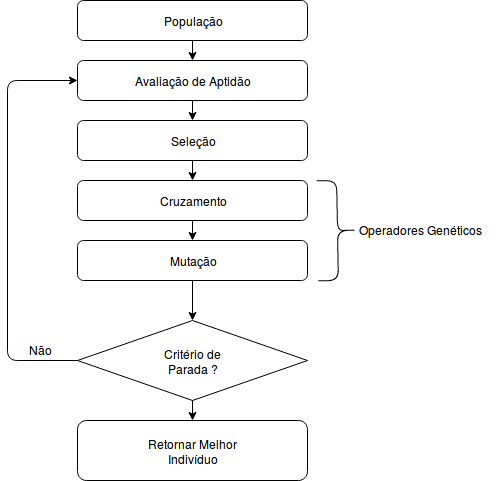
\includegraphics[scale=0.4]{algoritmo-genetico.png}}
    \caption{Estrutura básica de um algoritmo}
    \label{fig}
    \end{figure}
    
    Até o presente momento todos os fundamentos apresentados basearam-se na nos algoritmos genéticos simples. Existem outros tipos de algoritmos genéticos que foram desenvolvidos para problemas mais específicos.
    
\section{Metodologia Experimental}

Em geral, um AG possui duas categorias de parâmetros da pesquisa experimental: qualitativos e quantitativos. Os principais parâmetros qualitativos são os tipos de crossover (um ponto, dois pontos e múltiplos pontos) e os métodos de seleção (proporcional, escalonamento, Boltzmann, ranqueamento e tournament). Os principais parâmetros quantitativos são constituídos pelo tamanho da população (n), pela taxa de crossover (TC) e pela taxa de mutação (Tm). 

Para os experimentos realizados neste trabalho, utilizamos somente a metodologia quantitativa pois somente os parâmetros básicos foram alterados. Como por exemplo: tamanho da população, taxa de crossover e mutação além do tamanho do genótipo a ser encontrado.

Os objectivos da investigação quantitativa consistem essencialmente em encontrar relações entre variáveis, fazer descrições recorrendo ao tratamento estatístico dos dados recolhidos, testar teorias e tirar conclusões.

\section{Resultado e Discussão}

Na Tabela 1 estão resumidos os resultados dos experimentos realizados. Pode-se observar que as mudanças realizadas na taxa de crossover e mutação influenciam de forma significativa no número de iterações necessárias para encontrar o genótipo.  

Mas se esta for muito alta, estruturas com boas aptidões poderão ser retiradas mais rápida um valor alto, a maior parte da população será substituída, mas com valores muito altos pode ocorrer perda de estruturas de alta aptidão. Com um valor baixo, o algoritmo demorou um tempo maior para convergir.

    \begin {table}
    \caption {Resumo experimentos}
    \begin{center}
      \begin{tabular}{ l | c | r }
        \hline
        Indivíduos&	Tamanho Genótipo&	\% mutação&	\% Crossover&	# gerações médio&	Fitness médio \\ \hline
        20&	25&	1.00\%&	50.00\%&	3262.92&	13.50&  \hline
        20&	25&	2.00\%&	50.00\%&	6022.61&	13.16& \hline
        20&	25&	10.00\%&	60.00\%&	7410.37&	12.64& \hline
        20&	16&	1.00\%&	50.00\%&	143.75&	8.83&  \hline
        20&	16&	2.00\%&	50.00\%&	73.39&	8.72& \hline
        20&	16&	10.00\%&	60.00\%&	48.12&	8.20& 
        \hline
      \end{tabular}
      \end{center}
    \end{table}

Uma baixa taxa de mutação previne que uma dada posição fique estagnada em um valor, além de possibilitar que se chegue em qualquer ponto do espaço de busca. Com uma taxa muito alta a busca se torna essencialmente aleatória.
    
Vale ressaltar que o algoritmo de seleção utilizado nos experimentos foi o seleção por roleta. Quanto melhores são os cromossomos, mais chances de serem selecionados, mas por outro lado, existe a probabilidade da perda do melhor indivíduo.

\section*{Conclusão}

O principal objetivo deste trabalho foi entender o funcionamento de um algoritmo genético clássico e desenvolver uma solução que pudesse gerar novos indivíduos, até que um determinado genótipo fosse encontrado. Foram testados os efeitos dos parâmetros passados para o método de crossover, tamanho da população e taxa de mutação. Foi possível perceber que houve diferenças na quantidade de gerações necessárias para encontrar o genótipo, levando em consideração a quantidade de indivíduos, taxa de crossover e mutação.

O melhor desempenho do algoritmo genético é dependente da escolha de uma boa configuração de seus parâmetros.


\begin{thebibliography}{00}

\bibitem{b1} HOLLAND, J.H. Adaptation in Natural and Artificial Systems. Boston: MIT Press, 1992.
\bibitem{b2} BARCELLOS,  J.  C.  H. Algoritmos  genéticos  adaptativos:  um  estudo  comparativo. Dissertação  de mestrado. Universidade Estadual de São Paulo, Escola \bibitem{b3} Politécnica. São Paulo: 2000. Disponível em: http://www.portal.anchieta.br/revistas-e-livros/ubiquidade/pdf/artigo4.pdf
\bibitem{b4} IYODA, E. M. Inteligência Computacional no Projeto Automático de Redes Neurais Híbridas e  Redes  Neurofuzzy  Heterogêneas. Dissertação  (Mestrado)  —  \bibitem{b5} Universidade  Estadual  de Campinas  (Unicamp),  Campinas São  Paulo,  2000.  Disponível  em: <http://www.dca.fee.unicamp.br/~vonzuben/research/emi\_mest.html>
\bibitem{b6} POZO A. et. al. Computação Evolutiva. Universidade Federal do Paraná. Depto. de Informática. Diponível em: <http://www.inf.ufpr.br/~aurora/tutoriais/Ceapostila.pdf>
\bibitem{b7} (COSTA  FILHO  e POPPI,  1999) COSTA  FILHO, Paulo  Augusto  da;  POPPI,  RoneiJesus. Algoritmos  Genéticos em Química.  Química Nova. Campinas,  v. 22,  n.  3, jun.1999.  Disponível  em:  <http://www.scielo.br/pdf/qn/v22n3/1094.pdf>.
\end{thebibliography}
\vspace{12pt}

\end{document}
